\section{Serial Communication Interfaces}
\subsection{SPI (Serial Peripheral Interface)}$~$ \\
In einem SPI Netzwerk kann jeweils nur ein Master vorhanden sein. Jedoch ist es möglich, dass mehrere Slaves am selben Bus angeschlossen sind. Die folgenden Signale werden für die SPI Schnittstelle benötigt:
\begin{compactitem}
    \item \textbf{SCLK}: Taktsignal
    \item \textbf{MOSI / SDO}: Datensignal vom Master zum Slave.
    \item \textbf{MISO / SDI}: Datensignal vom Slave zum Master.
    \item \textbf{CS}: Signalisiert dem Slave eine aktive Kommunikation. Sind mehrere Slaves am selben Bus angeschlossen, so existiert oft für jeden Slave ein eigenes CS-Signal.
\end{compactitem}

\subsubsection{Taktpolarität und Taktphase}
Es gibt insgesamt vier SPI-Modi. Diese unterscheiden sich in der Taktpolarität und Taktphase.
\begin{figure}[H]
    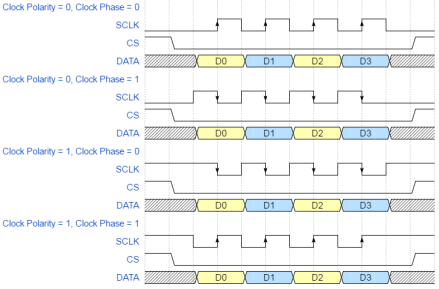
\includegraphics[width=0.5\textwidth]{images/spi_taktphase.png}
\end{figure}

\subsubsection{Timing}
Eine mögliche SPI Transaktion ist untenstehend zu sehen:
\begin{figure}[H]
    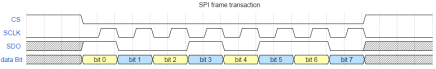
\includegraphics[width=1\textwidth]{images/spi_timing.png}
\end{figure}

\subsubsection{Hardwaremässige Implementierung}
Die Hardware für eine SPI Schnittstelle kann mittels zwei Schieberegistern (eines für das Senden, sowie eines für das Empfangen) realisiert werden.
\begin{multicols}{2}
    \begin{figure}[H]
        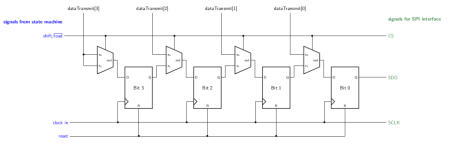
\includegraphics[width=0.5\textwidth]{images/spi_shift1.png}
    \end{figure}
    \begin{figure}[H]
        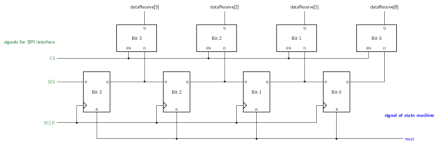
\includegraphics[width=0.5\textwidth]{images/spi_shift2.png}
    \end{figure}
\end{multicols}

\subsubsection{Implementierung in VHDL}
\lstinputlisting[language=VHDL,style=VHDL]{code/spiMaster.vhd}

\subsection{I\textsuperscript{2}C (Inter-Integrated Circuit)}$~$ \\
Das I\textsuperscript{2}C Interface ist ein bidirektionales Bussystem. Es können beliebig viele Master und Slaves angehängt werden. Die folgenden Signale werden für die I\textsuperscript{2}C Schnittstelle benötigt:
\begin{compactitem}
    \item \textbf{SCL}: Taktsignal
    \item \textbf{SDA}: Bidirektionales Datensignal
\end{compactitem}

\subsubsection{Übertragungsgeschwindigkeiten}
Die folgenden Geschwindigkeiten sind im I\textsuperscript{2}C Standard definiert:
\begin{compactitem}
    \item standard mode: 100 kbit/s
    \item fast-mode: 400 kbit/s
    \item fast-mode-plus: 1 Mbit/s
    \item high-speed mode: 3.4 Mbit/s
\end{compactitem}

\subsubsection{Timing}
Die folgenden Zustände auf dem I\textsuperscript{2}C Bus sind möglich:
\begin{figure}[H]
    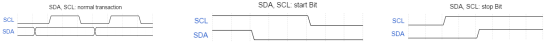
\includegraphics[width=1\textwidth]{images/i2c_bitstates.png}
\end{figure}
Eine mögliche I\textsuperscript{2}C Transaktion ist untenstehend zu sehen:
\begin{figure}[H]
    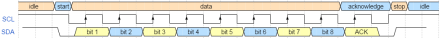
\includegraphics[width=1\textwidth]{images/i2c_timing.png}
\end{figure}
Nach dem Senden des Acknowledge-Bits, kann jeweils ein weiteres Byte gesendet werden, ohne die Transaktion durch Senden eines Stopbits zu unterbrechen. \\
Sollte ein Slave mehr Zeit brauchen um Daten zu verarbeiten, so kann er das SCL Signal auf Low ziehen, bis er wieder bereit ist.

\subsubsection{Arbitration}
Da mehrere Master und Slaves gleichzeitig senden könnten, ist eine Arbitrierung notwendig. Diese ist untenstehend dargestellt.
\begin{figure}[H]
    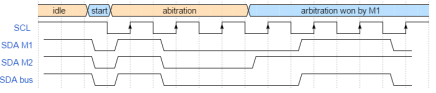
\includegraphics[width=0.75\textwidth]{images/i2c_arbitration.png}
\end{figure}
Der letzte Teilnehmer, welcher die SDA Leitung auf Low ziehen kann, gewinnt die Kommunikation.

\begin{multicols}{2}
    \subsubsection{Kommunikations Protokoll}
    \paragraph{Schreiben vom Master zum Slave}
    \begin{figure}[H]
        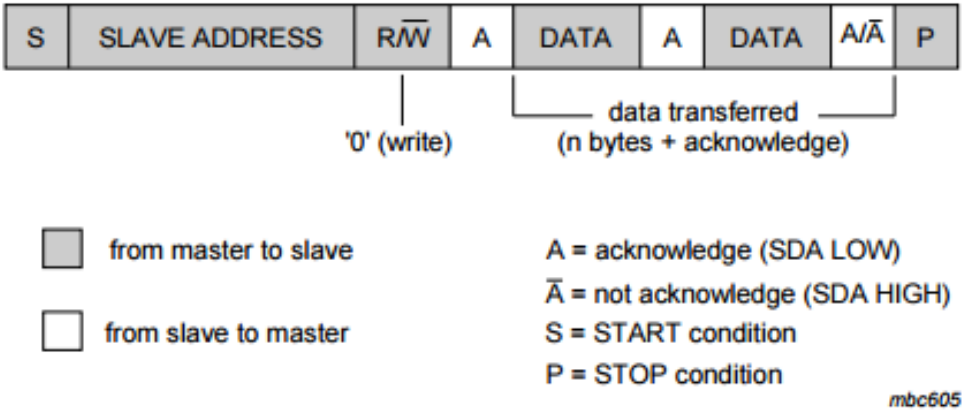
\includegraphics[width=0.5\textwidth]{images/i2c_protocolWrite.png}
    \end{figure}

    \paragraph{Lesen vom Slave}
    \begin{figure}[H]
        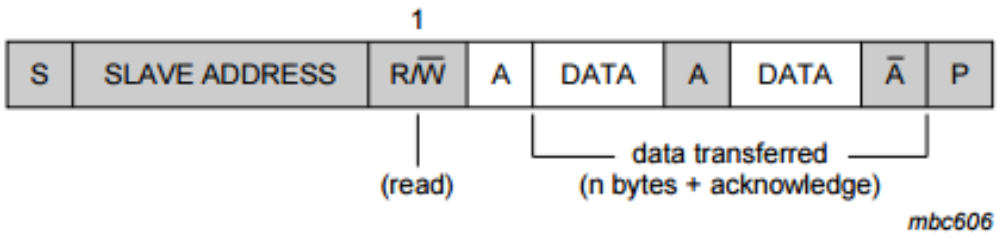
\includegraphics[width=0.5\textwidth]{images/i2c_protocolRead.png}
    \end{figure}

    \ \\ \ \\

    \subsubsection{Hardwaremässige Implementierung}
    Damit keine Kurzschlüsse entstehen, wenn zwei Master gleichzeitig senden wollen, werden die beiden Signale über externe Pull-Up-Widerstände auf einen High Pegel gezogen.
    \begin{figure}[H]
        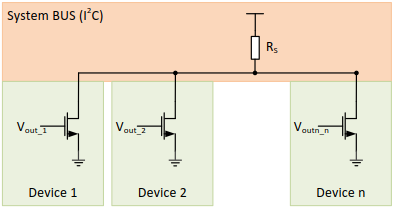
\includegraphics[width=0.5\textwidth]{images/i2c_hardware.png}
    \end{figure}
\end{multicols}

\subsubsection{Implementierung in VHDL}
Da die beiden I\textsuperscript{2}C-Signale bidirektional sind, muss in VHDL ein IO-Buffer für die beiden Signale instantiiert werden. Der nachfolgende Code instantiiert zwei solche Buffer.
\lstinputlisting[language=VHDL,style=VHDL]{code/i2cMaster.vhd}

\subsection{UART (Universal Asynchronous Receiver Transmitter)}$~$ \\
UART ist eine Punkt-zu-Punkt Schnittstelle. Es wird pro Richtung ein Datensignal benötigt.

\subsubsection{Timing}
Eine UART Transaktion startet immer mit einem Startbit. Anschliessend wird ein Datenbyte gesendet, eine Parität, sowie ein Stoppbit (oder mehrere Stopbits). Da kein Takt mitgesendet wird, muss im Sender und Empfänger die Geschwindigkeit bekannt sein.
\begin{figure}[H]
    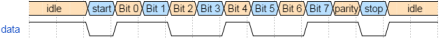
\includegraphics[width=0.75\textwidth]{images/uart_timing.png}
\end{figure}

\subsubsection{Hardwaremässige Implementierung}
\begin{figure}[H]
    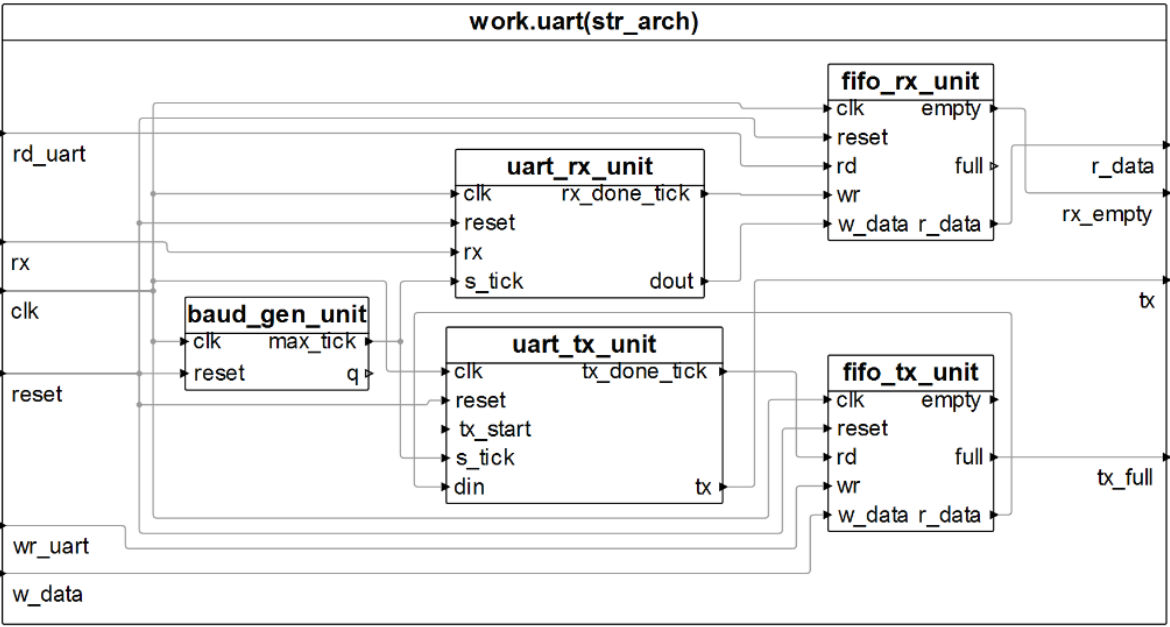
\includegraphics[width=0.75\textwidth]{images/uart_hardware.png}
\end{figure}

\subsubsection{VHDL Implementation}
\lstinputlisting[language=VHDL,style=VHDL]{code/uart.vhd}
